\documentclass[12pt,a4paper]{article}
\usepackage[utf8]{inputenc}
\usepackage[spanish,es-tabla]{babel}
\usepackage{amsmath}
\usepackage{amsfonts}
\usepackage{amssymb,latexsym,cancel}
\usepackage{graphicx}
\usepackage[left=2cm,right=2cm,top=2cm,bottom=2cm]{geometry}
\renewcommand{\baselinestretch}{1.5}
\usepackage{epstopdf}
\usepackage{subfigure}
\usepackage{array}
\usepackage{float}
\usepackage{longtable}
\newcolumntype{E}{>{$}c<{$}}
%%%%%%%%%%%%%%%%%%%%%%%%%%%
\usepackage{fancyhdr}
\pagestyle{fancy}
\fancyhead{}
\fancyhead[R]{ }
\fancyfoot[C]{\thepage}
\renewcommand{\headrulewidth}{0.9pt}
\renewcommand{\footrulewidth}{0.9pt}
\usepackage{url}


\begin{document}


\title{Actividad 1\\ Cambio climático  }
\author{
 Jorge Benz Olguín Aguilar\\
\small{División de Ciencias Exactas, Departamento de Física}\\
\small{Universidad de Sonora}\\
}
\date{\small{\today}}
\maketitle

%%%%%%%%%%%%%%%%%%%%%%%%%%%%%%%%%%%%%%%%%%%%%%%%%%%%%%%%%%%%%%%%%%%%%%%%%%%%%%%%%%%%%%%%%%%%%%%%%%%%%%%%%%%%%%%%%%

\section{Introducción}

\noindent La última década ha sido testigo de una sorprendente serie de tormentas, incendios forestales, sequías, decoloración de corales, olas de calor e inundaciones en todo el mundo con tan solo 1,8 grados Fahrenheit (1,0 grados centígrados) de calentamiento global.  Pero mucho de esto empeorará sustancialmente con 2,7 grados Fahrenheit de calentamiento, y mucho peor a 3,6 grados Fahrenheit (2 grados Celsius), según el "Informe especial del IPCC" sobre el calentamiento global de $1.5^{\circ} $C.

\noindent Si bien todos los países se comprometieron en virtud del Acuerdo de París a limitar el aumento de la temperatura global a $1.5^{\circ} $C-$2^{\circ} $C, quedaron las principales preguntas: ¿Cómo puede el mundo lograr este objetivo de temperatura? ¿Y qué pasa si no lo hace?
\noindent Los principales científicos del clima, el Panel Intergubernamental sobre el Cambio Climático (IPCC), respondieron estas preguntas y más en su último informe. Cerca de 100 científicos analizaron cómo el mundo puede lograr el objetivo de $1.5^{\circ} $C, así como los impactos asociados con este aumento de la temperatura.

\section{Síntesis}

\noindent Aquí hay ocho resultados:

\noindent 1. Limitar el calentamiento a $1.5^{\circ} $C requiere una transformación mayor e inmediata.

\noindent Las emisiones globales fueron de aproximadamente 52 GtCO2e en 2016, y se proyecta que sean de 52-58 GtCO2e para 2030. Las emisiones anuales deben ser aproximadamente la mitad de esa cantidad (25-30 GtCO2e / año en promedio) para 2030 para limitar el calentamiento a $1.5^{\circ} $C (con sin sobrepaso o bajo). Si bien aún es técnicamente factible evitar un aumento de temperatura de $1.5^{\circ} $C, el comportamiento y las tecnologías tendrán que cambiar de forma general para lograr estas reducciones de emisiones. Por ejemplo, para 2050, se proyecta que las energías renovables suministrarán el 70-85 por ciento de la electricidad en vías de $1.5^{\circ} $C. La eficiencia energética y las medidas de cambio de combustible serán críticas para el sector del transporte. Reducir la demanda de energía y mejorar la eficiencia de la producción de alimentos, cambiar las opciones dietéticas y reducir la pérdida y el desperdicio de alimentos también tienen un potencial significativo para reducir las emisiones.



\noindent 2. La escala de la transición baja en carbono requerida no tiene precedentes.

\noindent Si bien ha habido ejemplos de cambios rápidos en tecnologías o sectores específicos en el pasado, no hay precedentes en nuestra historia documentada para la tasa de cambio en la escala requerida para limitar el calentamiento a $1.5^{\circ} $C. En otras palabras, nunca antes hemos presenciado transiciones tan generalizadas y rápidas, y deberán realizarse a través de sistemas de energía, tierra, industriales, urbanos y otros, así como a través de tecnologías y geografías.

\noindent Hacer este cambio monumental requerirá nuevas inversiones sustanciales en tecnologías y eficiencia bajas en carbono. El informe encuentra que si se va a cumplir el objetivo de $1.5^{\circ} $C, las inversiones en tecnología de energía baja en carbono y eficiencia energética necesitarán incrementarse en aproximadamente un factor de cinco para 2050 en comparación con los niveles de 2015.

\noindent 3. "Limitar el calentamiento a $1.5^{\circ} $C" puede significar diferentes cosas, con diferentes resultados.

\noindent La mayoría (81 de 90) de los escenarios de modelado para limitar el calentamiento a $1.5^{\circ} $C excede este umbral de temperatura antes de volver a caer. Los resultados de estos escenarios son muy diferentes de aquellos que nunca superan los $1.5^{\circ} $C. Por ejemplo, considere los impactos del calentamiento en un ecosistema frágil: si se excede la meta de $1.5^{\circ} $C durante muchos años a una temperatura significativamente más alta, pueden producirse impactos irreversibles, como la extinción de las especies, incluso si el calentamiento finalmente se reduce a $1.5^{\circ} $C.

\noindent Los impactos de $1.5^{\circ} $C de calentamiento también dependerán de las actividades de reducción de emisiones elegidas. Por ejemplo, una reducción más rápida del carbono negro puede ayudar a detener la pérdida de nieve y hielo en el Ártico.

\noindent Además, es importante tener en cuenta que el objetivo de $1.5^{\circ} $C es el aumento de la temperatura promedio global. El aumento de la temperatura en cualquier ubicación, así como sus impactos resultantes, variará.

\noindent 4. Un límite de $1.5^{\circ} $C al calentamiento no es seguro para todos ...

\noindent El informe encuentra que los impactos climáticos significativos ya ocurren a $1.5^{\circ} $C, especialmente en áreas bajas, salud humana y océanos. Los impactos afectarán más a los pobres y más vulnerables debido a la pérdida de medios de subsistencia, la inseguridad alimentaria, el desplazamiento de la población, los efectos en la salud y más.

\noindent 5.… pero los riesgos asociados con el calentamiento son sustancialmente menores a $1.5^{\circ} $C que a $2^{\circ} $C.

\noindent Debido a que el Acuerdo de París especifica que los países deberían "limitar el calentamiento a muy por debajo de $2^{\circ} $C y realizar esfuerzos para limitarlo a $1.5^{\circ} $C", el informe del IPCC evalúa cuánto más altos son los riesgos de un mundo de $2^{\circ} $C que $1.5^{\circ} $C. Por ejemplo, a menos de $1.5^{\circ} $C de calentamiento, el informe encuentra que es muy probable que tenga un verano libre de hielo marino cada 100 años; a $2^{\circ} $C, la frecuencia aumenta a al menos uno cada 10 años.

\noindent 6. Las emisiones deberán alcanzar el cero neto a mediados de siglo.

\noindent Además de los grandes recortes de emisiones en la próxima década, las emisiones netas de CO2 en promedio deberán reducirse a cero a mediados de siglo. Si la fecha de alcanzar las emisiones netas cero se adelanta una década hasta 2040, a menos de 25 años, la posibilidad de limitar el calentamiento a $1.5^{\circ} $C es considerablemente mayor. Cuanto antes las emisiones alcancen su nivel máximo antes de 2030 y cuanto más bajo sea el nivel al que lo hagan, menos desafiantes serán los desafíos.

\noindent Deben abordarse todos los contaminantes que conducen al cambio climático. El informe señala el papel crítico de los contaminantes climáticos de corta duración pero altamente potentes, como el metano y los hidrofluorocarbonos (HFC). Si bien el dióxido de carbono domina el calentamiento a largo plazo, la reducción de otros contaminantes puede contribuir a la meta de $1.5^{\circ} $C en el corto plazo, con beneficios colaterales sustanciales, como la reducción de la contaminación del aire.

\noindent 7. Todas las vías de emisiones de $1.5^{\circ} $C dependen en cierta medida de la eliminación de carbono.

\noindent El informe muestra claramente que tendremos que centrar los esfuerzos no solo en reducir las emisiones, sino también en eliminar y almacenar el carbono de la atmósfera. La eliminación de carbono es necesaria tanto para pasar a emisiones netas nulas como para producir emisiones netas negativas para compensar cualquier exceso de $1.5^{\circ} $C. Las vías estudiadas en el informe dependen de diferentes niveles de remoción de carbono (que van desde 100-1,000 GtCO2 a lo largo del siglo XXI para escenarios con limitados o sin rebasamiento), pero todos confían en ello hasta cierto punto. El informe señala que la remoción de carbono implementada a tal escala no está comprobada, y es un riesgo importante para nuestra capacidad de limitar el calentamiento a $1.5^{\circ} $C. El informe también señala que la viabilidad y la sostenibilidad de la eliminación de carbono podrían mejorarse si se persigue una cartera de enfoques de eliminación de carbono.

\noindent 8. Todos, países, ciudades, el sector privado, individuos, deberán fortalecer su acción, sin demora.

\noindent Sin la transformación en la sociedad y la rápida implementación de los recortes ambiciosos de emisiones, limitar el calentamiento $1.5^{\circ} $C y lograr un desarrollo sostenible será extremadamente difícil, si no imposible. Incluso si los países cumplen con sus objetivos climáticos nacionales actuales y hacen grandes recortes de emisiones después de 2030, el calentamiento probablemente aún excederá los $1.5^{\circ} $C, dados los desafíos asociados con la reducción de emisiones a cero antes de 2045. Por lo tanto, todos los países y estados no estatales. Los actores deberán reforzar sus contribuciones sin demora. La decisión de la COP en París solicitó a los países que presenten un próximo conjunto de compromisos climáticos para 2020, por lo que esta es una oportunidad importante para tomar medidas más audaces. 

\noindent “Consecuencias sustanciales”

\noindent "Limitar el calentamiento global a $1.5^{\circ} $C en comparación con $2^{\circ} $C reduciría los impactos desafiantes sobre los ecosistemas, la salud humana y el bienestar", dijo Priyardarshi Shukla, Presidente del Centro Mundial para el Medio Ambiente y la Energía de la Universidad de Ahmedabad en la India. Autor del Informe Especial, en un comunicado. Dichos impactos incluyen tormentas más fuertes, clima más errático, olas de calor peligrosas, mares en ascenso e interrupciones a gran escala de la infraestructura y los patrones de migración.


\noindent En virtud del Acuerdo de París de 2015, todos los países del mundo acordaron mantener las temperaturas globales muy por debajo de los $2^{\circ} $C, mientras que los estados insulares de baja altitud y otros presionaron por mucho menos. Las promesas actuales para reducir las emisiones de CO2 elevarán el calentamiento global a al menos $3^{\circ} $C en 2100, lo que aumentará el riesgo de puntos de inflexión naturales, como la descongelación de grandes áreas de permafrost, lo que podría hacer que las temperaturas globales sean incontrolablemente más altas.

\noindent El calentamiento global es como estar en un campo minero que se vuelve cada vez más peligroso, dice Michael Mann, climatólogo y director del Centro de Ciencias del Sistema de la Tierra en Penn State. "Cuanto más avanzamos, más explosiones es probable que activemos: 1.5C es más seguro que 2C, 2C es más seguro que 2.5C, 2.5C es más seguro que 3C, y así sucesivamente", dijo Mann, quien no participó directamente en Este último informe del IPCC.

\noindent Además, dependiendo de la rapidez con que se recortan las emisiones, es posible que entre 0,4 y 2,7 millones de millas cuadradas (1-7 millones de kilómetros cuadrados) de tierra se conviertan en cultivos de bioenergía y hasta 3,86 millones de millas cuadradas (10 millones de kilómetros cuadrados) De los bosques añadidos para 2050. Y aún así eso no será suficiente, advierte el informe. Cada libra de CO2 emitida en los últimos cien años continuará atrapando el calor en la atmósfera durante los próximos cientos de años. Para 2045 o 2050 todavía habrá demasiado CO2 en la atmósfera. Según el informe, más bosques o alguna forma de captura directa que saque el CO2 de la atmósfera será esencial para estabilizar las temperaturas globales a 2,7 grados Fahrenheit (1,5 grados Celsius).

\noindent Los bosques también podrían desempeñar un papel mucho más importante en la reducción de las emisiones, dice Deborah Lawrence, experta en bosques de la Universidad de Virginia. "Los bosques brindan un servicio súper importante para la humanidad al eliminar actualmente alrededor del 25 por ciento de nuestro CO2", dijo Lawrence en una entrevista.

\noindent La reforestación y la mejora de la gestión forestal en conjunto podrían eliminar el CO2 de la atmósfera, dijo Lawrence, que representa un 18 por ciento de las reducciones necesarias para 2030. Brasil, China, India, México, Australia, Estados Unidos, Rusia y la Unión Europea también podrían aumentar sustancialmente Un estudio de próxima aparición demostrará que sus bosques son económicos y sin afectar la producción de alimentos, mientras que potencialmente eliminan miles de millones de toneladas de CO2 de la atmósfera, dijo Lawrence. Proteger e incrementar los bosques tropicales es especialmente importante ya que enfrían el aire y son clave para crear precipitaciones regionales para el cultivo de alimentos.

\noindent Cuando la madera de los bosques maduros se convierte en muebles o edificios, el CO2 se puede almacenar a largo plazo, dijo. Esa es una de las razones por las que un edificio de madera de 12 pisos se completará en Portland en 2019, y un edificio de madera de 24 pisos se está construyendo en Viena, Austria.

\noindent Los bosques existentes deben protegerse para evitar un cambio climático peligroso, advierte una coalición de científicos forestales en una declaración. Los bosques del mundo contienen más carbono que los depósitos explotables de petróleo, gas y carbón, señalan.

\noindent "El clima futuro de nuestro planeta está inextricablemente vinculado al futuro de sus bosques", escribieron los científicos.


\section{México}

\noindent Pero, como andamos en México, a continuación presentamos una imagen que muestra las emisiones de $CO_2$ de varios países, donde podremos hacer un comparativo y darnos cuenta donde estamos con respecto a los demás países

\begin{figure}[H]
  \centering
   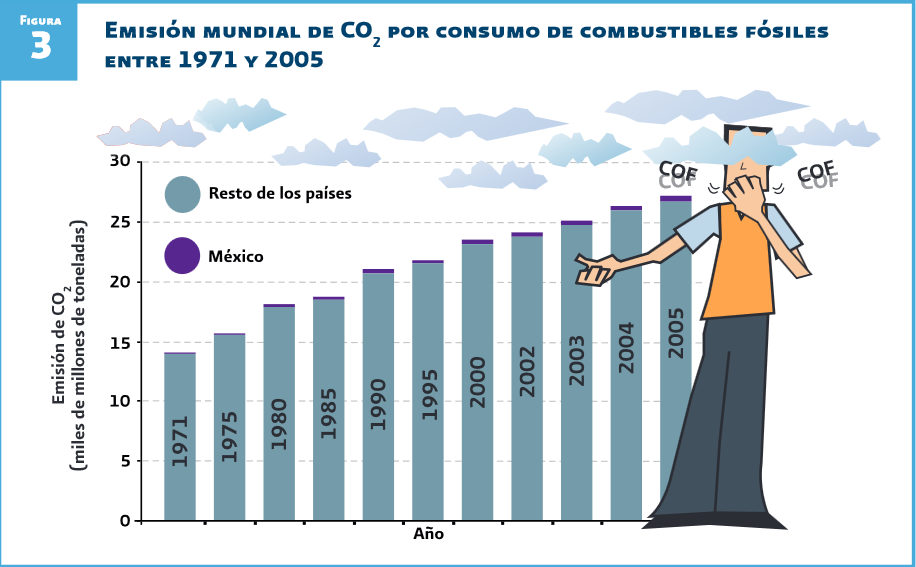
\includegraphics[scale=0.8]{grafica1.PNG}
  \caption{Emisiones de $CO_2$}
  \label{fig:ejemplo}
\end{figure} 

\noindent Ahora  veamos  qué  cantidad  de  GEI  emitimos en  México.  De  acuerdo  con  el  último  Inventario Nacional   de   Emisiones   de   Gases   de   Efecto Invernadero,  en  2002  se  produjeron  poco  más de 553 millones de toneladas de GEI. Suena poco si lo comparas con la emisión mundial, pero en realidad no lo es tanto si consideras que el peso de los GEI que se emiten en México equivale a unas 5 mil 500 veces el concreto empleado en la  construcción  del  Estadio  Azteca. 

\noindent El  panorama resulta  más  preocupante  si  consideramos  que nuestras  emisiones  se  han  incrementado  en  los últimos años: la emisión del 2002 fue 30\% mayor que la estimada doce años antes, en 1990.En el 2002, la principal fuente de gases de efecto invernadero  en  México  fue  el  sector  energía, responsable  de  cerca  de  70\%  de  las  emisiones. En  este  sector  se  incluye  el  consumo  de  los combustibles fósiles, indispensable para mover los autos y otros transportes y para la generación de electricidad.\cite{3} 

\begin{figure}[H]
  \centering
   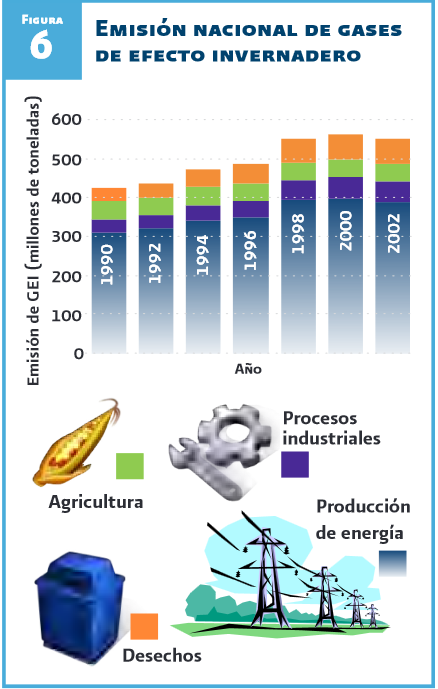
\includegraphics[scale=0.8]{grafica2.PNG}
  \caption{Emisiones de $CO_2$}
  \label{fig:ejemplo}
\end{figure} 

\noindent Los estudios que se presentaron en el informe son muy alarmantes y precisan acciones inmediatas, no podemos permitir que el planeta se siga degradando al ritmo en que lo que está haciendo. Es necesario que la gente tome conciencia sobre el gran problema que enfrentamos; ya que, de lo contrario, nos tocara lamentar lo que no hicimos y que podíamos haber hecho para vivir en un mundo mejor.  Un gran problema para llegar a la meta deseada es que vivimos en un mundo muy desigual; por un lado tenemos a los países desarrollados, con la posibilidad de migrar a tecnologías mas amigables con el medio ambiente y, por otra parte, los países pobres, los cuales siempre estarán supeditados a adquirir las tecnologías que les impongan los que la tengan. Difícil situación.

\begin{thebibliography}{0}

\bibitem {1} https://www.wri.org/blog/2018/10/8-things-you-need-know-about-ipcc-15-c-report

\bibitem {2} https://www.nationalgeographic.com/environment/2018/10/ipcc-report-climate-change-impacts-forests-emissions/

\bibitem{3} https://www.conafor.gob.mx/biblioteca/cambio-climatico-09-web.pdf


\end{thebibliography}


\end{document}







